\label{chapt:standards}

Before any complex analysis is completed, initial existing codes and standards will be investigated.\\

The most important parameter in question is the outer diameter $D_o$. For this entire report, it will be assumed that this value is constant at $D_o = 711\ mm = 28\ in$. Based on this fixed parameter, the following relevant values which will be used in this report are summarized below in Table~\ref{table:prelim_params}. All material properties selected as per John Umina's  suggestion from Table 1A of \cite{ASMEbvpcIID} for a SA-106 Grade B steel (most commonly used in seamless pipe). Units shown in both metric (SI) and United States customary (USC).\\

\begin{table}[ht]
	\caption{Key drum parameters and material properties.}
	\centering
	%	\begin{tabular}{c c c c}
	%		%heading
	%		\hline \textbf{Description} & \textbf{Symbol} & \textbf{Value} & \textbf{Units}\\[1 ex]
	%		\hline
	%		%Main table body content	
	%		Outer diameter		&$D_o$			& $28$		& $in$ 	\\
	%		Tether diameter		&$D_{thr}$		& $0.6$		& $in$ 	\\
	%		Drum length			&$L$			& $49$		& $in$ 	\\
	%		Tether tension		&$T$			& $11,525$	& $lbf$	\\	
	%		Yield strength		&$S_y$			& $35,000$	& $psi$	\\	
	%		Young's Modulus		&$E$			& $2.9\cdot 10^7$ &$psi$\\
	%		Poisson's ratio		&$\nu$			& $0.3$		& $ul$	\\	
	%		\hline
	%	\end{tabular}
	\begin{tabular}{lccccc}
		&       & \multicolumn{2}{c}{\textbf{\textit{SI}}} & \multicolumn{2}{c}{\textbf{\textit{UCS}}} \\
		\textbf{Description} & \textbf{Symbol} & \textbf{Value} & \textbf{Units} & \textbf{Value}  & \textbf{Units} \\
		\midrule
		Outer diameter       & $D_o$           & $711.2$        & $mm$           & $28$            & $in$           \\
		Tether diameter      & $D_{thr}$       & $15.2$         & $mm$           & $0.598$         & $in$           \\
		Drum length          & $L$             & $1,244.6$      & $mm$           & $49$            & $in$           \\
		Tether tension       & $T$             & $51,264$       & $N$            & $11,525$        & $lbf$          \\
		Yield strength       & $S_y$           & $241.3$        & $MPa$          & $35,000$        & $psi$          \\
		Young's modulus      & $E$             & $200$          & $GPa$          & $2.9\cdot 10^7$ & $psi$          \\
		Poisson's ratio      & $\nu$           & $0.3$          & $-$            & $-$             & $-$            \\
		Safety factor        & $SF$            & $1.5$          & $-$            & $-$             & $-$            \\
	\end{tabular}%
	\label{table:prelim_params}
\end{table}

The best approach to this problem is to model the drum as an externally pressured vessel. First, in order to make this approximation, it is required to investigate how the tether tension is translated into an external pressure. This will be done by reviewing the derivation for the Capstan Equation.\\ 

Next, using the above mentioned parameters and pressure, it was suggested by John Umina that the following standards should be investigated.
\begin{itemize}
	\item American Society of Mechanical Engineers (ASME):
	      \begin{itemize}[label=$\bullet$]
	      	\item Boiler and Pressure Vessel Code, Section VIII, Division 1, 2015 \cite{ASMEbvpcVII1}
	      	\item Boiler and Pressure Vessel Code, Section VIII, Division 2, 2015 \cite{ASMEbvpcVII2}
	      \end{itemize}
	\item European Standard EN
	      \begin{itemize}[label=$\bullet$]
	      	\item EN 13445: Unfired Pressure Vessels, Part 3: Design,  2002 \cite{EN134453}
	      \end{itemize}
	\item Det Norske Veritas(DNV)
	      \begin{itemize}[label=$\bullet$]
	      	\item DNV-OS-D101, Marine and Machinery Systems and Equipment \cite{DNVOSD101}
	      \end{itemize}
	\item Thin Walled Pressure Vessel (TWPV) Hoop Stress \cite{roarks}\\	
\end{itemize}

It is to be noted that the same symbols used in the aforementioned references will be used in the foregoing sections for clarity.
%----------------------------------------------------------------------------------------------------------------------
\section{Capstan Equation}
It is required to understand how one wrap of tether in tension results in an external pressure $p$ applied to the outer surface of the cylinder.\\

After much research into this problem, the solution reveals itself into the derivation of the well-known Capstan Equation~\ref{eq:Capstan} \cite{capstanman}.

\begin{equation}
	\label{eq:Capstan}
	T_2 = T_1 e^{\mu\theta}
\end{equation}

Where $T_1$ is the hold force and $T_2$ is the pull force (i.e. $T_2 \geq T_1$). \\

From this equation, the free body diagram that leads to this solution is presented below in Figure~\ref{fig:Capstan}~\cite{capstanman}. 

\begin{figure}[H]
	\centering
	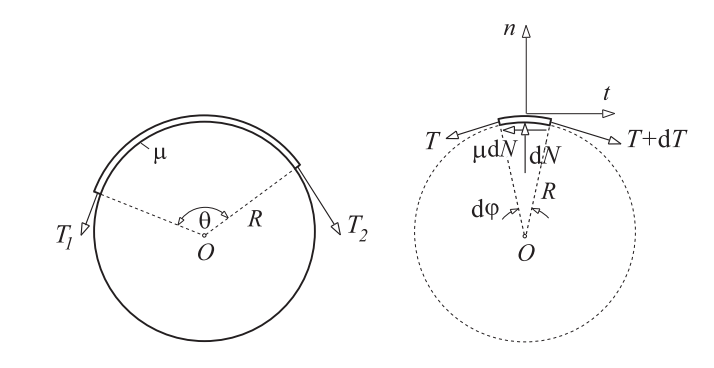
\includegraphics[scale=0.75]{2_Capstan}
	\caption[Free body diagram of differential capstan problem.]{Free body diagram of differential capstan problem. \protect\cite{capstanman}}
	\label{fig:Capstan}
\end{figure}

Based on this, what is of question is how to extrapolate a pressure $p$ from the applied tension $T$. This can be done performing a force balance ($\Sigma F_{\hat{n}} = 0 $)in the normal direction $\hat{n}$ which reduces to Equation~\ref{eq:CapstanSigRad}.

\begin{equation}
	\label{eq:CapstanSigRad}
	dN-(T+dT)\sin \frac{d\varphi}{2}+T\sin \frac{d\varphi}{2}= 0
\end{equation}

By assuming a small change in angle, the substitution of $\sin \varphi \approx \varphi$ and $dT d\varphi/2 \approx 0$ are be made. Applying these relations to \ref{eq:CapstanSigRad} leaves \ref{eq:diffNormal}.

\begin{equation}
	\label{eq:diffNormal}
	dN = T d\varphi
\end{equation}

%%-----------------------------

Similarly, a force balance ($\Sigma F_{\hat{t}} = 0 $)in the tangential direction $\hat{t}$ which reduces to Equation~\ref{eq:CapstanSigTan}.

\begin{equation}
	\label{eq:CapstanSigTan}
	(T+dT)\cos \frac{d\varphi}{2}- T\cos \frac{d\varphi}{2} - \mu dN= 0
\end{equation}

Again, assuming a small change in angle ($\cos \varphi \approx 1$) to \ref{eq:CapstanSigTan} leads to \ref{eq:diffTens}.

\begin{equation}
	\label{eq:diffTens}
	dT = \mu dN
\end{equation}

From the above equation, it is now clear that the overall normal force $N$ caused by the tension $T$ can be solved for by integration \ref{eq:capstan_integral} yielding \ref{eq:CapstanNorm}.

\begin{equation}
	\label{eq:capstan_integral}
	\int_0^N dN =\int_0^{2\pi} T d\varphi
\end{equation}

\begin{equation}
	\label{eq:CapstanNorm}
	N=2\pi T	
\end{equation}

With this resultant normal force over one revolution of tether, it is now apparent that the pressure $p$ can be solved for by distributing $N$ over this area as seen in Equation~\ref{eq:2_preq}.

\begin{equation}
	\label{eq:2_preq}
	p=\frac{N}{A}=\frac{2\pi T}{d\pi D}=\frac{2T}{Dd}
\end{equation}

Using the values from Table~\ref{table:prelim_params} and \ref{eq:2_preq}, $p=1376\  psi= 9.484\  MPa$. 

%------------------------------------------------------------------------------------------
\subsection{Alternate Solution}
\label{subsection:alt}
By letting $T = T(\theta)= T_{hi} e^{-\mu \varphi}$, Equation~\ref{eq:capstan_integral} becomes \ref{eq:capstan_integral2} hence yielding \ref{eq:CapstanNorm2} (recall $\int e^{ax} dx = \frac{1}{a} e^{ax} + C$).

\begin{equation}
	\label{eq:capstan_integral2}
	\begin{aligned}
		\int_0^N dN =\int_0^{\theta} T_{hi} e^{-\mu \varphi} d\varphi            \\
		N = \left( -\frac{T_{hi}}{\mu} e^{-\mu \varphi} \right) \Big|_0^{\theta} 
	\end{aligned}
\end{equation}

\begin{equation}
	\label{eq:CapstanNorm2}
	N = \frac{T_{hi}}{\mu} \left( 1 - e^{-\mu \theta} \right)
\end{equation}

With this stored normal force, it is now the pressure $p$ after $\theta$ of contact angle,  can be solved for by distributing $N$ over this area (dependent on angle) as seen in Equation~\ref{eq:2_preq2}.

\begin{equation}
	\label{eq:2_preq2}
	p=\frac{N}{A}= \frac{T_{hi} \left( 1 - e^{-\mu \theta} \right)}{\mu d_{thr} R \theta}
\end{equation}

Using a script from Appendix~\ref{appendix:a0}, the following plots in Figures~\ref{fig:2_nvar} and \ref{fig:2_pvar} show the variation in normal force $N$ and pressure $p$ for different values of coefficient of friction $\mu$.

\begin{figure}[H]
	\centering
	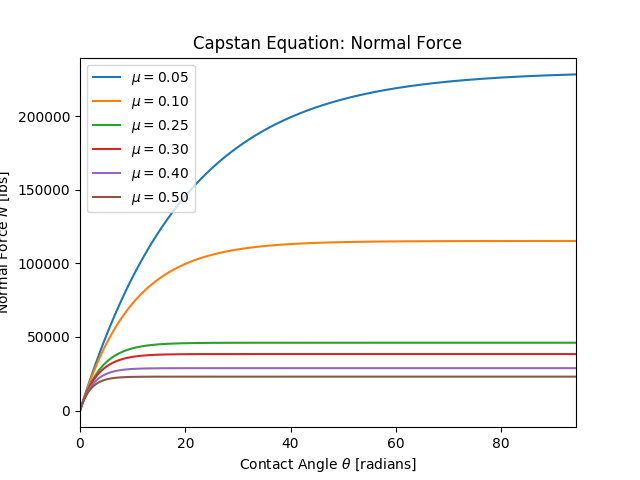
\includegraphics[scale=0.75]{2_nvar}
	\caption{Variation of stored normal force $N$ versus contact angle $\theta$.}
	\label{fig:2_nvar}
\end{figure}

\begin{figure}[H]
	\centering
	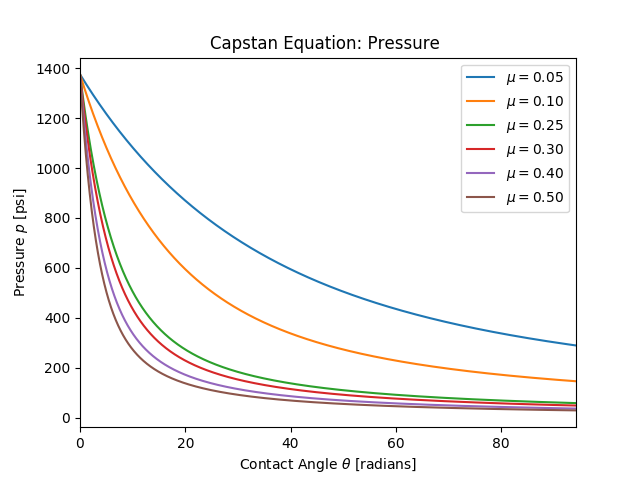
\includegraphics[scale=0.75]{2_pvar}
	\caption{Variation of pressure $p$ versus contact angle $\theta$.}
	\label{fig:2_pvar}
\end{figure}

It is clear from these plots that as the contact angle increases, the stored normal force has an asymptomatic behavior. This behavior coupled with the increase increase in area results in a pressure which goes to zero. Furthermore, as the coefficient of friction between the tether and the drum increases, the decay in pressure is quicker. A key observation to be made is that regardless of the $\mu$, all initial pressures $p(\theta)$ start at the value calculated from Equation~\ref{eq:2_preq}.  

%%----------------------------------------------------------------------------------------------------------------------
\section{ASME's BPVC}

The ASME codes listed in the beginning of this chapter will be extensively studied. Note that for all iteration procedures in this report, an initial thickness of $t_0 = 12.7\ mm=0.500\ in$ with a step of $t_0 = 0.254\ mm=0.01\ in$. Python scripts utilized for implementing solving algorithms can be found in Appendix~A developed with \cite{PYTHON}. 
\subsection{Section VIII: Division 1}
As per UG-28 of \cite{ASMEbvpcVII1}, the following procedure was used to calculate the required thickness.
The following list of steps were carried out as per \cite{ASMEbvpcVII1}.

\begin{enumerate}
	\item Assume initial thickness value of $t$
	\item Calculate $D_o/t$ ratio and assure $D_o/t \geq 10$.
	\item Calculate $L/D_o$ ratio, if $L/D_o \geq 50 \Rightarrow 50$ or  $L/D_o \leq 0.05 \Rightarrow 0.05$
	\item With above ratios, go to Figure G of \cite{ASMEbvpcIID} and get value for $A$
	\item With $A$ from above go to chart CS-2 $\because S_y \geq 30 \ ksi$ to get $B$
	\item Use Equation \ref{eq:2_VII1_pa} with $B$ to calculate allowable pressure $p_a$:
	      \begin{equation}
	      	\label{eq:2_VII1_pa}
	      	p_a = \frac{4B}{3 \left(D_o/t\right)}
	      \end{equation}
	\item Check that $p_a \geq p_{req}$ as calculated from Equation~\ref{eq:2_preq}, if not, increase $t$ and go to Step 2\\
	      	
\end{enumerate}

With the Python Script from Appendix~\ref{appendix:a1} the convergence plot from Figure~\ref{fig:2_vii1_cnvg} below was created.
\begin{figure}[H]
	\centering
	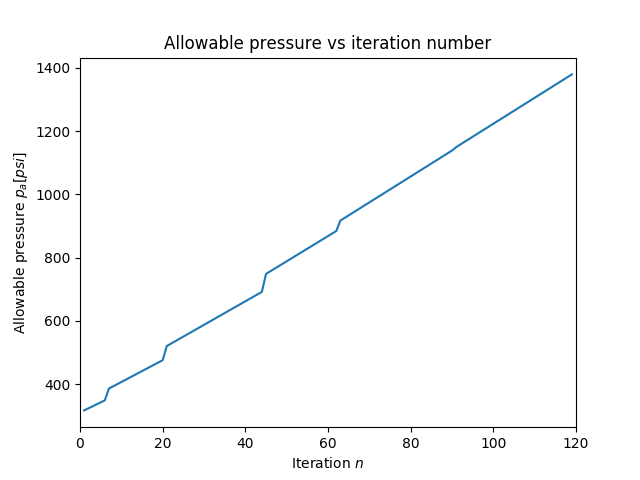
\includegraphics[scale=0.8]{2_vii1_cnvg}
	\caption{Convergence plot of $p_a$ using ASME's BPVC VIII-1.}
	\label{fig:2_vii1_cnvg}
\end{figure}

From this plot, the script converged at thickness of $t = 43.7\ mm = 1.68\ in$ and an allowable pressure of $p_a\geq p_{reqs}$ after $n=119$ iterations. 


\subsection{Section VIII: Division 2}
As per subsection 4.4.5 of \cite{ASMEbvpcVII2}, the following procedure was used to calculate the required thickness. Note that only the main formulas will be presented. For intermediate steps, see  the Python script in Appendix~\ref{appendix:a2}. The following list of steps were carried out as per \cite{ASMEbvpcVII2}.

\begin{enumerate}
	\item Assume initial thickness value of $t$
	\item Calculate elastic buckling stress $F_{he}$ with Equation~\ref{eq:2_VII2_4419}
	      \begin{equation}
	      	\label{eq:2_VII2_4419}
	      	F_{he} = \frac{1.6\ C_h E_y t}{D_o}
	      \end{equation}
	\item Based on $S_y$ and $F_{he}$, calculate the predicted buckling stress $F_{ic}$ \ref{eq:2_VII2_4419}
	\item With subsection 4.4.2 of \cite{ASMEbvpcVII2}, compute the design factor $FS$
	\item Calculate allowable pressure $p_a$ with Equation~\ref{eq:2_VII2_4428}
	      \begin{equation}
	      	\label{eq:2_VII2_4428}
	      	p_a = 2 F_{ha} \left(\frac{t}{D_o}\right)
	      \end{equation}
	\item Check if $p_a \geq p_{req}$ as calculated from \ref{eq:2_preq}, if not, increase $t$ and go to Step 2 \\
	      	
\end{enumerate}

%%on page~\pageref{fig:2_vii2_cnvg} for page ref
The Python Script in Appendix~\ref{appendix:a2} output the following convergence plot as seen in Figure~\ref{fig:2_vii2_cnvg}.
\begin{figure}[H]
	\centering
	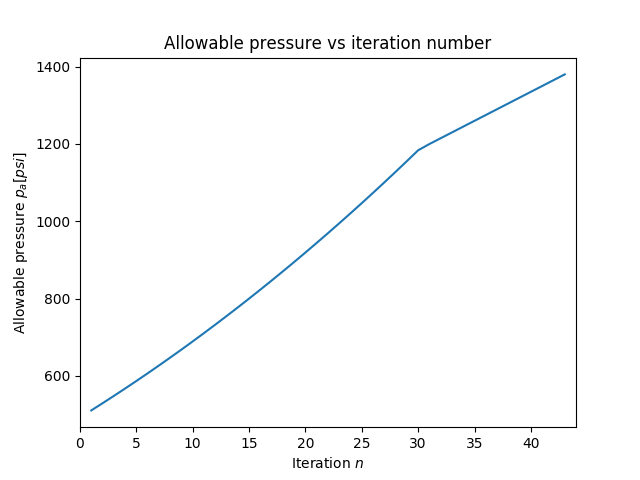
\includegraphics[scale=0.8]{2_vii2_cnvg}
	\caption{Convergence plot of $p_a$ using ASME's BPVC VIII-2.}
	\label{fig:2_vii2_cnvg}
\end{figure}

Convergence was reached at a thickness of $t = 23.4\ mm = 0.920\ in$ when $p_a\geq p_{req}$, after $n=43$ iterations. 


%%----------------------------------------------------------------------------------------------------------------------
\section{European Standard}
\subsection{EN-13445-3}
As per subsection 8.5.2.2 of \cite{EN134453}, the following procedure was used to calculate the required thickness $e_a$. Note that the script in Appendix~~\ref{appendix:a3} utilizes SI units as per \cite{EN134453}.

\begin{enumerate}
	\item Assume initial thickness value of $e_a$ and calculate $p_y$ with \ref{eq:2_EN_py}
	      \begin{equation}
	      	\label{eq:2_EN_py}
	      	p_y = \frac{\sigma_e e_a}{R}
	      \end{equation}
	\item Compute the lower failure pressure $p_m$ \ref{eq:2_EN_pm}, see 8.5.2.6 of \cite{EN134453} for $\varepsilon$
	      \begin{equation}
	      	\label{eq:2_EN_pm}
	      	p_m = \frac{E e_a  \varepsilon}{R}
	      \end{equation}
	\item With the $p_m/p_y$ ratio, use Figure 8.5.5 of \cite{EN134453} to find equivalent $p_r/p_y$
	\item Rearrange for $p_r$ and calculate allowable pressure $p$ ith \ref{eq:2_EN_pa}
	      \begin{equation}
	      	\label{eq:2_EN_pa}
	      	p = \frac{p_r}{S}
	      \end{equation}
	\item Check if $p \geq p_{req}$ as calculated from \ref{eq:2_preq}, if not, increase $e_a$ and go to Step 2\\
\end{enumerate}

Again, with the respective Python Script in Appendix~\ref{appendix:a3}, a convergence plot was created (see Figure~\ref{fig:2_en13445_cnvg}).
\begin{figure}[H]
	\centering
	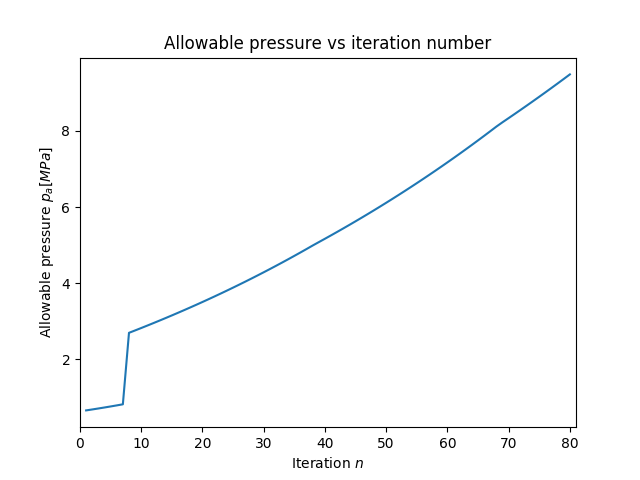
\includegraphics[scale=0.8]{2_en13445_cnvg}
	\caption{Convergence plot of $p_a$ using EN 13445-3.}
	\label{fig:2_en13445_cnvg}
\end{figure}

The script converged at thickness of $e_a = 32.8\ mm = 1.290\ in$ and an allowable pressure of $p\geq p_{req}$ after $n=80$ iterations. 

%%----------------------------------------------------------------------------------------------------------------------
\section{DNV}

\subsection{DNV-OS-D101}

As per \cite{DNVOSD101}, in subsection F215, Equation~\ref{eq:2_DNV_hoop} is presented as follows.

\begin{equation}
	\label{eq:2_DNV_hoop}
	\sigma_h = C\cdot\frac{T}{d_{thr}t}
\end{equation}

In this equation, $C$ is a factor based on the number of wraps on the drum,. for two layers $C=1.75$ \cite{DNVOSD101}. There are a few exceptions with this equation and they are listed as follows.

\begin{enumerate}
	\item The hoop stress $\sigma_h$ is limited to $\sigma_h \leq 0.85\cdot S_y$
	\item The calculated $\sigma_h$  if superseded with larger tested value\\
\end{enumerate}

Rearranging Equation~\ref{eq:2_DNV_hoop} for $t$, setting $\sigma_h = S_{allow}=S_y/SF$ (see Table~\ref{table:prelim_params}) and solving accordingly will yield a valid value of $t = 36.6\ mm = 1.440 \ in$. 

%----------------------------------------------------------------------------------------------------------------------
\section{TWPV Hoop Stress}

Using the well known hoop stress equation \cite{roarks} for a TWPV, Equation~\ref{eq:2_hoop} is presented as follows.

\begin{equation}
	\label{eq:2_hoop}
	\sigma_h = \frac{pR}{t}
\end{equation}

Again, rearranging for $t$ , $\sigma_h = S_{allow}=S_y/SF$ and using the pressure $p$ calculated in \ref{eq:2_preq}, solving accordingly will yield a valid value of $t = 21.0\ mm = 0.825 \ in$. Note that $\because R/t = 17 \geq 10$, the assumption of a TWPV is valid.

%%----------------------------------------------------------------------------------------------------------------------
\section{Comparison}

Based on the above sections, the results are summarized in Table~\ref{table:2_comp}.
\begin{table}[H]
	\centering
	\caption{Comparison $t$ according to method used.}
	\begin{tabular}{lccc}
		\textbf{Method}  & \textbf{$\mathbf{mm}$} & \textbf{$\mathbf{in}$} & \textbf{SF} \\
		\midrule
		ASME BPVC VIII-1 & $43.7$                 & $1.680$                & $1.5$       \\
		ASME BPVC VIII-2 & $23.4$                 & $0.920$                & $1.5$       \\
		EN 13445-3       & $32.8$                 & $1.290$                & $1.5$       \\    
		DNV-OS-D101      & $36.6$                 & $1.440$                & $1.5$       \\
		TWPV Hoop Stress & $21.0$                 & $0.825$                & $1.5$       \\
	\end{tabular}%
	\label{table:2_comp}%
\end{table}%

Based on these results the following observations may be made

\begin{itemize}
	\item ASME's BPVC VIII-1 is the most conservative
	\item TWPV Hoop Stress and ASME's BPVC VIII-2 yield the least conservative results
	\item Both EN 13445-3  and DNV-OS-D101 are somewhere in between \\
\end{itemize}

Now that there is a benchmark for the expected values, a more analytically approach will be taken in the following section.